\documentclass[a4paper,12pt,final]{report}
\usepackage[margin=0.8in]{geometry}
% Pour une impression recto verso :
%\documentclass[a4paper,11pt,twoside,final]{article}
%%%%% Packages %%%%%
\usepackage[english]{babel}  % Rapport en français
\usepackage[utf8]{inputenc}   % UTF-8 forever <3
\usepackage[T1]{fontenc}      % font encoding (allows accents)
\usepackage[pdftex]{graphicx} % gestion des images
\usepackage{setspace}         % gestion des interlignes
\usepackage{csquotes}         % For quotes
\usepackage[hidelinks]{hyperref}         % gestion des url
\usepackage{titlesec}         % override chapter title
\usepackage{geometry}         % gestion des marges
\usepackage{float}            % Gestion des positionnement d'image
\usepackage[final]{pdfpages}  % Inclusion de fichier pdf
\usepackage{framed}
\usepackage{geometry}
%\usepackage{apacite}

%%% Affichage de code
\usepackage{listings}
\usepackage{xcolor}
\usepackage{textcomp}
\definecolor{comment}{rgb}{0.12, 0.38, 0.18 } % adjusted, in Eclipse: {0.25, 0.42, 0.30 } = #3F6A4D
\definecolor{keyword}{rgb}{0.37, 0.08, 0.25}  % #5F1441
\definecolor{string}{rgb}{0.06, 0.10, 0.98} % #101AF9
\lstset{
  columns=flexible, %prevent extra spaces
  rulecolor=\color{black!50},
  backgroundcolor = \color{blue!10},
  numbers=none, % line numbering
  showspaces=false,
  showtabs=false,
  tabsize=2,
  breaklines=true,
  showstringspaces=false,
  breakatwhitespace=false,
  commentstyle=\color{comment},
  keywordstyle=\color{keyword},
  stringstyle=\color{string},
  basicstyle=\ttfamily,
  extendedchars=true,
  emph=[2]{In},
  emphstyle=[2]\color{black!70},
  morecomment=[l][\color{blue}]{Out},
  frame=single,
  frameround=tttt,
  framerule=0.3pt,
  framesep=4pt,
  belowcaptionskip=2.1pt,
  literate={à}{{\`a}}1 {à }{{\`a} }1 {â}{{\^a}}1 %           letter a
           {À}{{\`A}}1 {Â}{{\^A}}1 %                         letter A
           {ç}{{\c{c}}}1 %                                   letter c
           {Ç}{{\c{C}}}1 %                                   letter C
           {é}{{\'e}}1 {è}{{\`e}}1 {ê}{{\^e}}1 {ë}{{\"e}}1 % letter e
           {É}{{\'E}}1 {È}{{\`E}}1 {Ê}{{\^E}}1 {Ë}{{\"E}}1 % letter E
           {î}{{\^i}}1 {ï}{{\"i}}1 %                         letter i
           {Î}{{\^I}}1 {Ï}{{\"I}}1 %                         letter I
           {ô}{{\^o}}1 %                                     letter o
           {Ô}{{\^O}}1 %                                     letter O
           {œ}{{\oe}}1 %                                     letter oe
           {Œ}{{\OE}}1 %                                     letter OE
           {ù}{{\`u}}1 {û}{{\^u}}1 {ü}{{\"u}}1 %             letter u
           {Ù}{{\`U}}1 {Û}{{\^U}}1 {Ü}{{\"U}}1 %             letter U
  % above is a hack to force UTF8 compatibility (only for french)
}


%%% Bibliographie
\usepackage[backend=biber,style=numeric-comp]{biblatex}
\addbibresource{7-bibliographie.bib}
%\bibliographystyle{plain}
%\bibliography{bibliographie}
%%%%% Configuration %%%%%
\definecolor{shadecolor}{gray}{0.9}

%\pagenumbering{arabic}

%%% Quelques champs
\newcommand{\reportsubject}{Gestion et optimisation du reporting au sein d'un projet de transport}  % Internship purpose
\newcommand{\reportauthor}{Lucas \textsc{LAMY}} % Author
\newcommand{\reportdates}{3 Septembre 2018 - 15 Février 2019 (A18)} %Internship dates
\newcommand{\reportdetails}{Lusail LRT - Thales Gulf (Qatar)} %Internship details
\newcommand{\reporttitle}{Rapport de stage - TN09 - GI} % Title
\renewcommand\labelitemi{---} %list items hyphens rather than nodes
\renewcommand{\contentsname}{Sommaire} % Nom table des matières
%%% Inline comment
\newcommand{\ignore}[1]{}

%%% Modification de style pour \chapter
\titleformat{\chapter}{\normalfont\huge}{\textbf{\thechapter.}}{20pt}{\huge\bf}

%%% Marges
\geometry{hmargin=2.45cm}

% Set line width
\newcommand{\HRule}{\rule{\linewidth}{0.5mm}}
% Espace entre les paragraphes
\setlength{\parskip}{1ex}

%% ToC Name :

\addto\captionsenglish{
  \renewcommand{\contentsname}
    {Sommaire} 
    \renewcommand{\listfigurename}{Table des figures}
}

%%% Meta-données
\hypersetup{
    pdftitle={\reporttitle},%
    pdfauthor={\reportauthor},%
    pdfsubject={\reportsubject},%
    pdfkeywords={Thales}{Qatar}{TN09}
    colorlinks=false,% hyperlinks will be black
    linkbordercolor=black,% hyperlink borders will be black
    pdfborderstyle={/S/U/W 1}% border style will be underline of width 1pt
}

%% Table of content configuration
\setcounter{tocdepth}{1}


\usepackage[toc,section=chapter]{glossaries}    % Glossaire

\makeglossaries

\newglossaryentry{TC}
{
	name=\underline{T\&C},
	description={\textit{Testing \& Commissioning}, département d'un projet dédié à l'inspection et à la mise en service des divers équipements et systèmes du projet}
}

\newglossaryentry{StAT}
{
	name=\underline{StAT},
	description={\textit{Stand Alone Test}, test unitaire, où l'équipement testé est isolé de toute interaction durant le test, afin de restreindre les critères du test à son fonctionnement autonome  }
}

\newglossaryentry{LRT}
{
	name=\underline{LRT},
	description={\textit{Light Rail Transit}, forme de transport en commun urbain ferroviaire disposant généralement d'une capacité et d'une vitesse inférieures à celles d'un train ou d'un métro, mais supérieures à celles des systèmes traditionnels de tramway. (c.f  \underline{\href{https://fr.wikipedia.org/wiki/Métro_léger}{Wikipédia}})}
	}

\newglossaryentry{TCS}
{
	name=\underline{TCS},
	description={\textit{Tramway Control System}, Système de Contrôle du Tramway}
}

\newglossaryentry{RST}
{
	name=\underline{RST},
	description={\textit{Rolling Stock}, ensemble du matériel roulant, ici c'est l'ensemble des différentes rames du LRT}
}

\newglossaryentry{PSD}
{
	name=\underline{PSD},
	description={\textit{Platform Screen Door}, portes palières ou encore façades de quai sont des portes automatiques vitrées situées le long des quais en bordure des voies ne s'ouvrant que lorsque la rame est à l'arrêt en station (c.f  \underline{\href{https://fr.wikipedia.org/wiki/Porte_palière_(métro)}{Wikipédia}})}
}

\newglossaryentry{ECS}
{
	name=\underline{ECS},
	description={\textit{Environmental Control System}, Système de Contrôle Environnemental}
}

\newglossaryentry{TVS}
{
	name=\underline{TVS},
	description={\textit{Tunnel Ventilation System},  Système de Ventilation des Tunnels }
}

\newglossaryentry{CCS}
{
	name=\underline{CCS},
	description={\textit{Communication and Control System}, Système de Contrôle et de Communication, département du projet concernant principalement les télécommunications, la sécurité et le monitoring}
}

\newglossaryentry{TETRA}
{
	name=\underline{TETRA},
	description={\textit{Terrestrial Trunked Radio}, système de radio numérique mobile professionnel bi-directionnel, spécialement conçu pour des services officiels et pour l'armée. Un réseau de type TETRA offre un canal radio partagé ouvert en permanence, et réservé à un groupe d'utilisateurs. Ceci permet d'établir une communication immédiate entre un utilisateur sur le terrain et un dispatcher, ou un groupe d'utilisateurs (c.f \underline{\href{https://fr.wikipedia.org/wiki/Terrestrial_Trunked_Radio}{Wikipédia}})}
}

\newglossaryentry{DTS}
{
	name=\underline{DTS},
	description={\textit{Digital Transmission System}, Système de Transmission Digitale, ensemble des différentes infrastructures réseau}
}

\newglossaryentry{COMTV}
{
	name=\underline{COMTV},
	description={\textit{Commercial Television}, Télévision commerciale, désigne l'ensemble des écrans situés en station et à bord des rames ayant pour fonction de diffuser des annonces publicitaires aux usagers}
}

\newglossaryentry{UPS}
{
	name=\underline{UPS},
	description={\textit{Uninterruptible Power Supply}, L'Alimentation Sans Interruption (ASI), ou encore un onduleur, est un dispositif de l'électronique de puissance qui permet de fournir un courant alternatif stable et dépourvu de coupures ou de microcoupures, quoi qu'il se produise sur le réseau électrique (c.f \underline{\href{https://fr.wikipedia.org/wiki/Alimentation_sans_interruption}{Wikipédia}})}
}


\newglossaryentry{PIS}
{
	name=\underline{PIS},
	description={\textit{Passenger Information System}, Système d'Information des Passagers automatisé permettant de leur fournir à la fois des informations statiques comme des tables horaires ainsi que des informations dynamiques comme l'attente avant la prochaine rame ou encore les incidents survenus sur le réseau (c.f \underline{\href{https://en.wikipedia.org/wiki/Passenger_information_system}{Wikipédia}})}
}

\newglossaryentry{PAS}
{
	name=\underline{PAS},
	description={\textit{Public Address System}, désigne un système d'amplification et de distribution sonore électronique par le biais d'un microphone, amplificateur et de haut-parleurs, permettant à une personne de communiquer un message (pré-enregistré ou en direct) au grand public (c.f \underline{\href{https://en.wikipedia.org/wiki/Public_address_system}{Wikipédia}})}
}

\newglossaryentry{ACS-IDS}
{
	name=\underline{ACS-IDS},
	description={\textit{Access Control System-Intrusion Detection System}, Système de Contrôle des Accès ainsi que de Détection des Intrusions}
}

\newglossaryentry{FDS}
{
	name=\underline{FDS},
	description={\textit{Fire Detection System}, Système de Détection des Incendies}
}

\newglossaryentry{CCTV}
{
	name=\underline{CCTV},
	description={\textit{Closed-Circuit Television}, Système de Vidéosurveillance}
}

\newglossaryentry{SCADA}
{
	name=\underline{SCADA},
	description={\textit{Supervisory Control And Data Acquisition}, Système de Contrôle et d'Acquisition de Données, système de télégestion à grande échelle permettant de traiter en temps réel un grand nombre de télémesures, d'informations visuelles (caméras par exemple), d'alarmes, de contrôler à distance des installations techniques}
}

\newglossaryentry{MMS}
{
	name=\underline{MMS},
	description={\textit{Maintenance Management System}, Système de Management de la Maintenance}
}

\newglossaryentry{AFC}
{
	name=\underline{AFC},
	description={\textit{Automatic Fare Collection}, Système de Collection Automatique des Billets}
}

\newglossaryentry{WA}
{
	name=\underline{WA},
	description={\textit{Wifi Access}, Système permettant de proposer aux usager du LRT de bénéficier d'un accès à Internet via un un réseau WiFi}
}

\newglossaryentry{SnagR}
{
	name=\underline{SnagR},
	description={Solution en ligne permettant l'édition et la gestion des rapports de test ainsi que des différents défauts présents sur les systèmes du projet }
}


\newglossaryentry{Mezzoteam}
{
	name=\underline{Mezzoteam},
	description={Base de données regroupant l'ensemble des documents produits par les différents acteurs du projet}
}

\newglossaryentry{e-TOL}
{
	name=\underline{e-TOL},
	description={Plateforme de gestion de projet et de partage de fichiers interne à Thales, permettant par exemple de partager des fichiers entre l'équipe basée en France (offshore) et l'équipe basée à Lusail (inshore)}
}

\newglossaryentry{reporting}
{
	name=\underline{reporting},
	description={Ensemble des processus permettant d'aboutir à la présentation des activités du projet et de leurs avancements. Ici ce terme est utilisé pour désigner la gestion de la production des rapports de test}
}

\newglossaryentry{KPI}
{
	name=\underline{KPI},
	description={\textit{Key Performance Indicator}, Indicateur clé de performance, indicateur graphique et/ou numérique permettant d'évaluer l'avancement d'un projet, de communiquer, de diagnostiquer les points bloquants ou encore de s'assurer de la continuité du progrès}
}

\newglossaryentry{RAMS}
{
	name=\underline{RAMS},
	description={\textit{Reliability Availability Maintainability and Safety}, en français : FMDS (Fiabilité Maintenabilité Disponibilité et Sécurité), entité en charge de la sûreté de fonctionnement au sein d'un projet}
}

\newglossaryentry{IDE}
{
	name=\underline{IDE},
	description={\textit{Integrated Development Environment} en français :  Environnement de Développement Intégré (EDI) }
}

\newglossaryentry{LaTeX}
{
	name=\underline{LaTeX},
	description={LaTeX est un langage de description donnant à l'auteur les moyens d'obtenir des documents mis en page de façon professionnelle sans avoir à se soucier de leur forme. La priorité est donnée à l'essentiel : le contenu (c.f \underline{\href{https://openclassrooms.com/fr/courses/1617396-redigez-des-documents-de-qualite-avec-latex/1617565-quest-ce-que-latex}{OpenClassrooms}})}
}

\newglossaryentry{Git}
{
	name=\underline{Git},
	description={logiciel de gestion de versions décentralisé. C'est un logiciel libre créé par Linus Torvalds, auteur du noyau Linux, et distribué selon les termes de la licence publique générale GNU version 2.  (c.f \underline{\href{https://fr.wikipedia.org/wiki/Git}{Wikipédia}})}
}

\newglossaryentry{PCR}
{
	name=\underline{PCR},
	description={\textit{Product Change Request}, requête formulée par un ingénieur, souvent par le biais d'un outil de gestion, afin de demander des changements dans le design d'un système}
}

\newglossaryentry{methodesagiles}
{
	name=\underline{méthodes agiles},
	description={Les méthodes agiles sont des groupes de pratiques de pilotage et de réalisation de projets. Elles ont pour origine le manifeste Agile, rédigé en 2001, qui consacre le terme agile pour référencer de multiples méthodes existantes. (c.f \underline{\href{https://fr.wikipedia.org/wiki/Méthode_agile}{Wikipédia}})}
}

\newglossaryentry{scraping}
{
	name=\underline{scraping},
	description={Le web scraping (parfois appelé harvesting) est une technique d'extraction du contenu de sites Web, via un script ou un programme, dans le but de le transformer pour permettre son utilisation dans un autre contexte. (c.f \underline{\href{https://www.luxury-concept.com/dev-blog/346-le-scaping-des-donnees-pourquoi-et-comment.html}{LuxuryConcept}})}
}

\newglossaryentry{TestCases}
{
	name=\underline{Test Cases},
	description={en français : scénarios de test, éléments composant les test, définis au moment du design afin de simuler plusieurs situations d'utilisation des systèmes de manière à prouver leur conformité vis à vis de toutes les exigences du cahier des charges}
	}

\newglossaryentry{SIT}
{
	name=\underline{SIT},
	description={\textit{Site Integration Test}, test d'intégration, ayant pour but de détécter les erreurs non détéctables pendant les test unitaires (c.f StAT). Ce type de test consiste à assembler différents composants afin de tester leur fonctionnement dans l'ensemble}
	}	
	
\newglossaryentry{E2E}
{
	name=\underline{E2E},
	description={\textit{End to End Test}, test bout en bout ayant pour but de vérifier si un système se comporte comme prévu du début à la fin. Le testeur doit se mettre dans le rôle d’un utilisateur et effectuer les tests comme s’il utilisait véritablement l’outil mis à sa disposition (c.f \underline{\href{https://blog.testingdigital.com/quest-test-de-bout-bout-end-to-end-1288}{TestingDigital}})}
	}

\newglossaryentry{SC}
{
	name=\underline{Safety Case},
	description={document indexant l'ensemble de exigences liées à la sécurité}
	}
	
\newglossaryentry{SIL}
{
	name=\underline{SIL},
	description={\textit{Safety Integrity Level}, niveau d'intégrité de sécurité, niveau relatif de réduction de risques inhérents à une fonction de sécurité, ou comme spécification d'une cible de réduction de risque. Plus simplement, c'est une mesure de la performance attendue pour une fonction de sécurité. (c.f \underline{\href{https://fr.wikipedia.org/wiki/Safety_Integrity_Level}{Wikipédia}})}
}

\newglossaryentry{API}
{
	name=\underline{API},
	description={\textit{Application Programming Interface }, Interface de Programmation Applicative, permettant à un logiciel d'offrir un accès facilité à certaines de ses fonctions, méthodes et classes}
}



\glsaddall




\pagenumbering{gobble}
%%%%% Début du document %%%%%
\begin{document}
\nocite{*}
\makeatletter
  \begin{titlepage}
    \centering
    \noindent
\includegraphics[height=0.8cm]{ressources/images/logos/Thales_Logo.png}\hfill
\includegraphics[height=1cm]{ressources/images/logos/logo_UTC.png}\\
    \vfill

    \textsc{\Large \reporttitle}\\[0.5cm]
    \HRule \\[0.4cm]
    {\huge \bfseries \reportsubject}\\[0.4cm]
    \HRule \\[1.5cm]
    \textsc{\large \reportdetails}\\[0.5cm]
    \textsc{\large \reportdates}\\[0.5cm]

    \vfill

    \begin{minipage}[t]{0.3\textwidth}
      \begin{flushleft} \large
        \emph{Auteur :}\\
        \reportauthor
      \end{flushleft}
    \end{minipage}
    \begin{minipage}[t]{0.6\textwidth}
      \begin{flushright} \large
        \emph{Superviseurs :} \\
		Vincent \textsc{ARGENTON}
		\linebreak
		Stéphane \textsc{GLOAGUEN} 
		\linebreak
		\emph{Suiveur :} \\
		Mohamed \textsc{SALLAK} 
    
      \end{flushright}
    \end{minipage}
  \end{titlepage}

\makeatother

\setstretch{1,3}
\chapter*{Remerciements} %the * make the chapter invisible in the table of content

Je tiens à remercier toutes les personnes qui ont contribué au succès de mon stage et qui m'ont aidé lors de la rédaction de ce rapport.  \\

Tout d'abord, je tiens à remercier vivement Mr Vincent ARGENTON, mon maitre de stage, pour le temps qu'ils m'a toujours accordé sans hésitation, ainsi que pour les opportunités et responsabilités qu'il m'a offert. \\

	Ensuite, je voudrais remercier le manager de l'équipe, Mr Stéphane GLOAGUEN, pour la reconnaissance, le temps et les conseils qu'il m'a accordé. \\
	
	De plus, je souhaite aussi remercier Kevin HELOUART, qui, avec Vincent, a su m'intégrer à l'équipe très rapidement.  \\

Enfin, je remercie Mr Michelangelo NERI et Mr Milan RADOVIC d'avoir accepté ma candidature.

Je souhaite aussi remercier tout mes collègues pour le temps passé à leurs côtés, ainsi que pour leurs précieux conseils.
%%%%% Faire Table des Figures
\setstretch{1,15}
\tableofcontents
\chapter*{Table des figures} %the * make the chapter invisible in the table of content
\addcontentsline{toc}{chapter}{Table des figures}

\begin{itemize}
\item \textbf{Figure 1 :} Dates clefs du groupe Thales - page 2
\item \textbf{Figure 2 :} Chiffres du groupe Thales en 2017 - page 4
\item \textbf{Figure 3 :} Vues satellites de la ville de Lusail entre 2006 et 2015 - source : http://www.lusail.com/whats-happening/construction-progress/satellite-images/2006-2/ - page 5
\item \textbf{Figure 4 :} Organigramme du projet du LRT de Lusail - page 6
\item \textbf{Figure 5 :} Organigrammes de l'équipe Thales au sein du projet du LRT de Lusail - pages 8 et 9
\item \textbf{Figure 6 :} Capture d'écran de l'outil Trello - page 13
\item \textbf{Figure 7 :} Processus initial - page 17
\item \textbf{Figure 8 :} Matrice RACl - page 18
\item \textbf{Figure 9 :} Processus final - page 18
\item \textbf{Figure 10 :} Capture d'écran de l'arborescence des sauvegardes- page 22
\item \textbf{Figure 11 :} Diagramme représentation l'organisation des données- page 25
\end{itemize}
\setstretch{1,3}
\chapter*{Résumé technique}
\addcontentsline{toc}{chapter}{Résumé technique}

Lors de mon TN09, j'ai effectué mon stage chez Thales Gulf, à Doha, au Qatar. Le projet auquel j'ai été affecté est un projet ferroviaire (\gls{LRT}) pour lequel Thales prend en charge la majorité des technologies de télécommunications. L'équipe \gls{TC}, dans laquelle j'ai évolué, est chargée de mettre en service et de tester les différents équipements des nombreux systèmes gérés par Thales. \\
Ma fonction principale était de rapporter l'avancement de la production des rapports de tests, afin, par exemple, de fournir des outils d'aide à la décision, ainsi que des indicateurs de progrès, à mes managers \\
Afin de mener à bien cette mission, j'ai utilisé 2 bases de données différentes. L'une regroupait tous les documents produits au cours du projet, l'autre permettait aux différentes équipes d'ingénieurs d'éditer et de stocker leurs rapports de tests. \\
Cependant, c'est sur la seconde base de données que la majorité de mon travail s'est concentrée. En effet, les informations indexées dans celle-ci correspondaient à une extraction des données brutes présentes dans les formulaires composant chaque rapport. Ainsi, un de mes projets fut de mettre au point un programme capable d'analyser ces données, les relier aux différentes variables , puis les intégrer au sein d'un fichier Excel afin de pouvoir fournir différentes statistiques et outils d'aide à la décision.\\
Lors de ce stage, j'ai pu découvrir de nombreuses structures d'entreprise ainsi que des domaines d'ingénierie informatiques divers et variés, mais aussi, comme vous pourrez le constater dans la suite de ce rapport, j'ai endossé de nombreuses responsabilités, qui ont contribuées à rendre cette expérience formatrice. \\
Dans ce rapport, je m'efforcerai de vous présenter le contexte de mon stage, la nature de mes missions, mes réalisations et enfin mon ressenti ainsi que l'expérience que j'en ai tirée.


\pagenumbering{arabic}
\chapter{Présentation générale}
\section{Le groupe Thales}
\subsection{Historique du groupe}

Le groupe Thales actuel est la résultante d'une évolution complexe,  jalonnée par plusieurs fusions dont voici les principales :
\begin{center}
\includegraphics[height=10cm]{ressources/images/figures/timeline.png}
\end{center}

\begin{itemize}
    \item \textbf{1968 :} La branche électronique de Thomson-Brandt et la Compagnie Générale de Télégraphie fusionne pour créer Thomson-CSF.
    \item \textbf{2000 :} Thomson-CSF fusionne avec Dassault Electronique et devient THALES. 
    \item \textbf{2007 :} Les activités d'Alcatel-Lucent liées au transport, à l'espace ainsi qu'à la sécurité sont transférées vers Thales par le biais d'une fusion, qui mène aussi à la création de Thales Alenia Space. 
    \item \textbf{2019 :} Après l'annonce en 2017 d'une offre de rachat de Gemalto, Thales a obtenu de la Commission Européenne la validation de l'OPA. Cette dernière devrait avoir lieu au premier trimestre de cette année. 
\end{itemize}

\subsection{Les domaines d'activités}

Thales est implantée dans 56 pays différents, et cela grâce à un large spectre de compétences, divisé en 5 secteurs d'activité qui sont :
\begin{itemize}
\item \textbf{La défense : }Thales est numéro 1 mondial dans la défense aérienne avancée et numéro 1 en Europe concernant l'électronique de défense. Les solutions conçues, déployées et maintenues par Thales concernent à la fois l'aérien, le terrestre, le spatial, le maritime ainsi que les communications radio, les systèmes interarmées et la cybernétique. 
\item \textbf{La sécurité :}En 2011, deux sociétés du groupe Thales fusionnent pour former Thales Communications \& Security dont les domaines d'activité sont multiples : la sécurité urbaine, la protection d'infrastructures critiques telles que les aéroports, la sécurité des systèmes de communication ainsi que la cybersécurité.
\item \textbf{L'aéronautique :}Thales domine le domaine de la gestion du trafic aérien, 2 tiers des avions possèdent à minima un équipement Thales que ce soit pour la navigation, la génération d'électricité, les solutions de divertissement ou encore les cockpits. 
\item \textbf{L'aérospatiale :}La présence du groupe dans l'aérospatiale civile et militaire est assurée par Thales Alenia Space,un des leader mondiaux dans la conception de satelites de communication. Cette société propose aussi des systèmes pour l'observation de la Terre, l'exploration,la navigation, le transport ainsi que les infrastructures spatiales (comme l'ISS).

\item \textbf{Les transports terrestres :}Thales élabore des solutions pour les grandes lignes ferroviaires mais aussi pour des moyens de transports urbains comme le métro, le tramway ou encore le \gls{LRT}.
Le groupe développe des solutions innovantes, fondées sur des technologies de pointe comme par exemple le Système Européen de Contrôle des Trains (ETCS).
\end{itemize}


\subsection{Position du groupe sur la scène internationale}

Voici les chiffres réalisés par Thales en 2017 :

\begin{center}
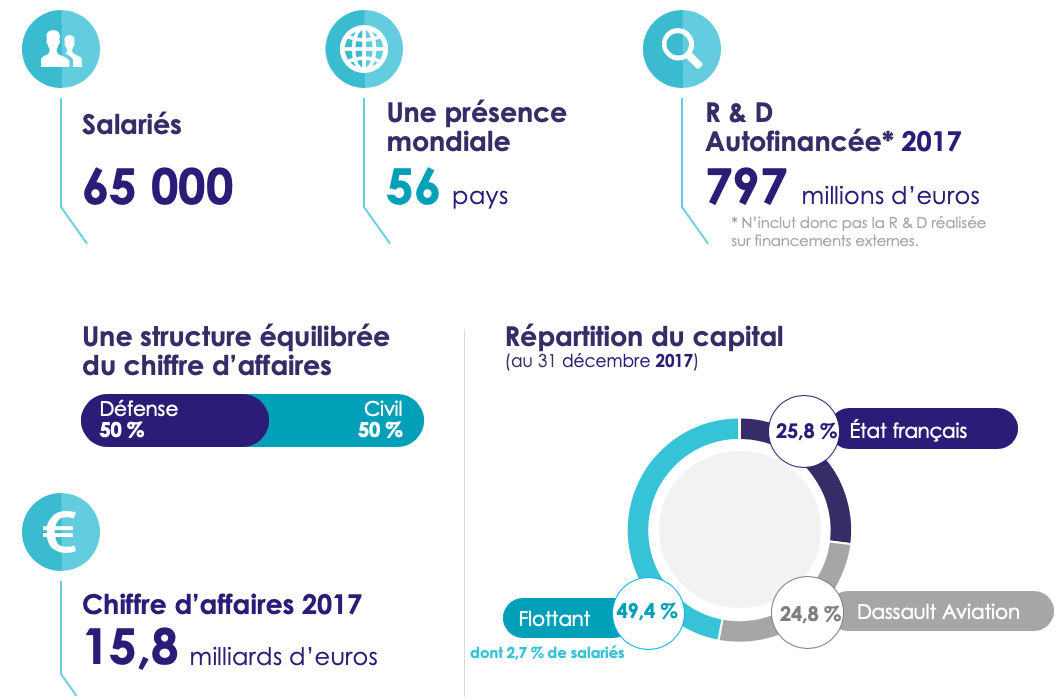
\includegraphics[height=8cm]{ressources/images/figures/Key.png}
\end{center}

En ce qui concerne la concurrence, Thales se positionne de la manière suivante : 
\begin{itemize}
\item \textbf{Pour la signalisation ferroviaire :} Même si Thales réalise tout de même un chiffre d'affaire annuel de 1,7 milliard d'euros, c'est son avance technologique dans le domaine des trains autonomes qui lui permettra de rivaliser avec le géant Siemens Alstom 
\item \textbf{Dans l'aéronautique :} Les 3 leader français dans ce domaine sont Thales, Safran et Zodiac. Ainsi Thales se partage le marché des équipementiers civil, mais possède une position de poids dans le secteur de l'aéronautique militaire et plus particulièrement dans la défense, notamment grâce à la part importante de son capital dédiée à la partie Dassault Aviation du groupe.
\end{itemize}

\section{Le projet : Lusail LRT}
\subsection{Le Light Rail Transit} Le Transit Léger sur Rail ou Métro léger, est une technologie de transport ferroviaire urbain. Sa vitesse moyenne et sa capacité de transport sont en général supérieures à celle d'un tramway mais inférieures à celles d'un métro. Le \gls{LRT} adopte le fonctionnement d'un métro sur les tronçons souterrains et celui du tramway sur ceux en surface.
Du point de vue du fonctionnement, la différence principale entre le \gls{LRT} et le métro réside dans le fait que plusieurs lignes différentes peuvent circuler sur des tronçons de voies communs. 
De nombreuses villes dans le monde ont déjà implanté un  \gls{LRT} dans leur réseau de transport en commun, telles que Hong Kong, Francfort, São Paulo, Ottawa ou encore Jérusalem.

\subsection{Le contexte du projet} Le projet se déroule dans la nouvelle ville de Lusail au Qatar située en périphérie de Doha, la capitale du pays. Cette ville, lorsqu'elle sera terminée, s'étendra sur 38 \begin{math} km^2 \end{math} et devrait accueillir 450 000 habitants. Elle tiendra une place centrale dans les activités culturelles, artistiques et sportives du pays avec par exemple le circuit international de Losail, mais aussi le stade de football qui accueillera le match d'ouverture et la finale de la Coupe du Monde de football. Dans l'optique de désengorger le trafic routier ainsi que de préparer au mieux l'accueil de la Coupe du Monde, la ville de Doha se verra équipée prochainement de 3 lignes de métro et la ville de Lusail se verra équipée de 4 lignes de LRT. Le projet concerné par ce rapport est celui du LRT de Lusail. Ce dernier comportera 4 lignes, 37 stations (dont 2 reliées aux réseau du métro de Doha), 28 rames pour une capacité totale de 50 000 voyageurs par jours.

\begin{center}
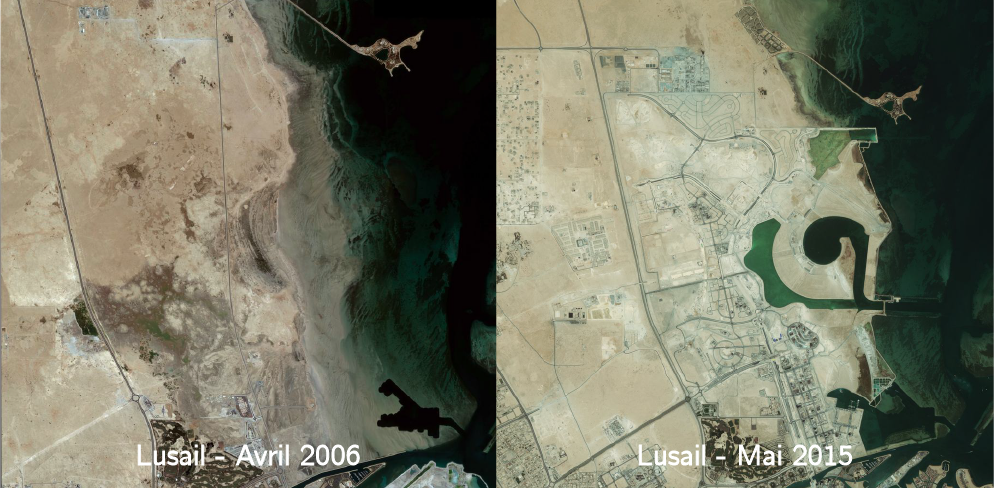
\includegraphics[height=8cm]{ressources/images/figures/Lusail.png}
\end{center}

\subsection{Les acteurs du projet}
De nombreuses entreprises sont impliquées sur ce projet de transport, puisque celui ci implique à la fois du génie civil, de l'ingénierie ferroviaire, des télécommunications ainsi que de la sécurité.
\begin{center}
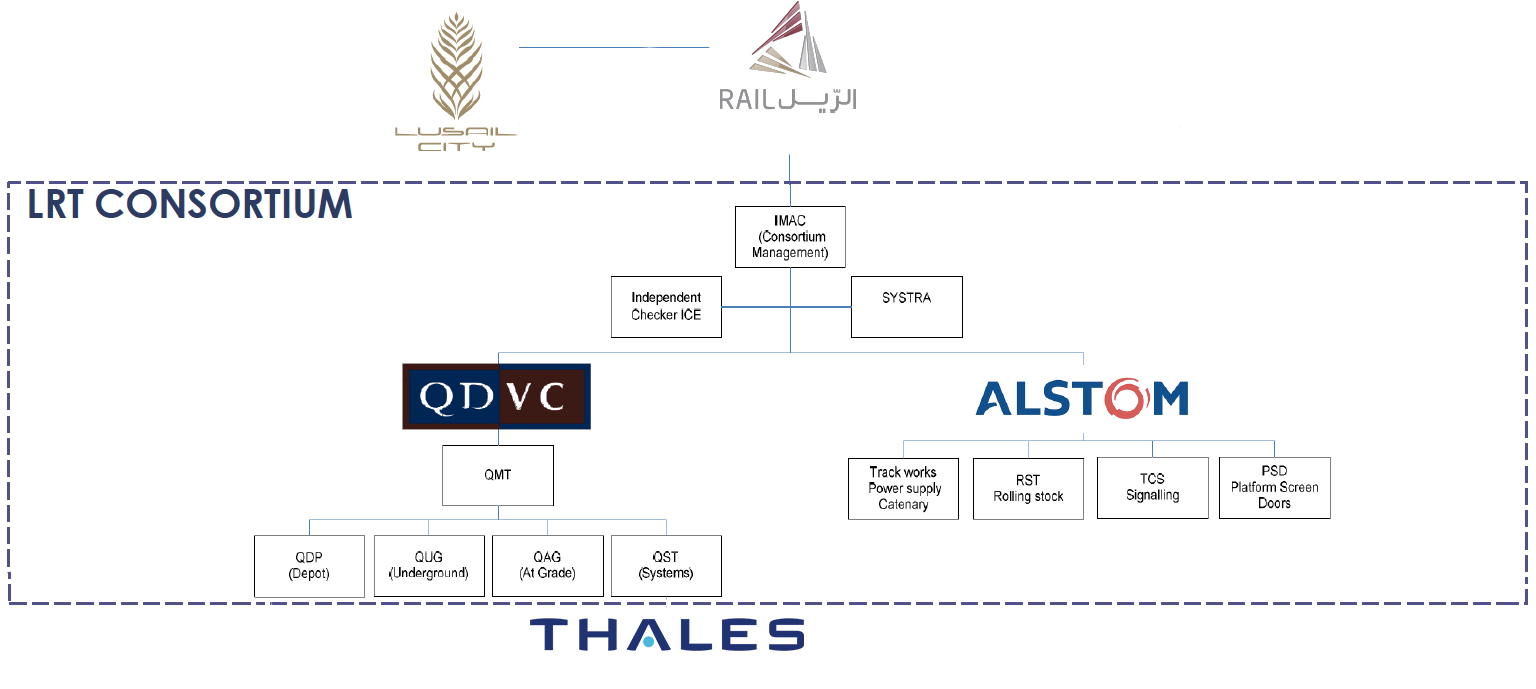
\includegraphics[height=8cm]{ressources/images/figures/Consortium.png}
\end{center}

\begin{itemize}
\item \textbf{Qatar Rail :} Entreprise crée après le début de la phase de définition du projet, afin de superviser l'ensemble du réseau ferroviaire du pays. C'est l'employeur et donc le client direct du Consortium. 
\item \textbf{IMAC :} Entité de management du consortium, elle est composée à la fois d'employés de QDVC et d'Alstom, les deux entreprises principales du consortium et fait l'intermédiaire entre le consortium et le client.
\item \textbf{ICE :} Entité de contrôle dont le rôle est assuré par la société SENER. Elle évolue de manière externe au consortium et donc indépendamment  de celui-ci afin de pouvoir certifier la conformité du système par rapport aux exigences du contrat au client Qatar Rails. 
\item \textbf{SYSTRA :} Entreprise réalisant pour l'IMAC des missions d'audit concernant le design. Elle est impliquée durant la phase de définition du projet en réalisant les différentes spécifications présentes dans le contrat mais aussi durant la phase de réalisation afin d'orienter les stratégies d'opération. 
\item \textbf{Alstom :} Alstom prends à charge toute la partie ferroviaire du projet : les rames (\gls{RST} : Matériel roulant), la signalisation (\gls{TCS} : Système de contrôle du tramway), les portes palières (\gls{PSD} : Portes palières) ou encore les caténaires. 
\item \textbf{QDVC :} QDVC est une  filiale à 51\% de Qatari Diar et à 49\% de VINCI Construction Grands Projets. Elle prends à charge notamment le génie civil pour les bâtiments du dépôt, les bâtiments sous-terrains ainsi que les bâtiments à la surface, que ce soit des stations ou des bâtiments techniques. Cette entreprise sous-traite trois secteurs d'activité :
\begin{itemize}
\item \textbf{\gls{CCS} :} Systèmes de contrôle et de communication, cette partie est assurée par Thales. 
\item \textbf{\gls{TVS} :} Système de Ventilation des Tunnels.
\item \textbf{\gls{ECS} :} Système de Contrôle Environnemental (température, humidité, etc)
\end{itemize}
\item \textbf{RKH :} Fruit de la fusion entre le consortium RATP Dev et Keolis (49\% ) et la société qatarie Hamad Group (51\%), RKH assurera l'exploitation et la maintenance du LRT de Lusail ainsi que du Métro de Doha.
\end{itemize}

\subsection{Place de Thales au sein du projet}

Sur ce projet, l'entreprise est positionnée en tant que sous-traitant de QDVC. Elle est en charge du design, de l'installation, des tests et de la mise en service des systèmes \gls{CCS}. Ces derniers sont organisés comme ceci :

\begin{itemize}
\item \textbf{Télécommunications :} Secteur d'activité clé de Thales, il représente une part importante du projet.
\begin{itemize}
\item \textbf{\gls{DTS} :} Système de Transmission Digitale, ensemble des différentes infrastructures réseau.
\item \textbf{Téléphonie :} Ce secteur englobe les téléphones présents dans les ascenseurs, dans les centres opérationnels ou encore la gestion de la téléphonie embarquée dans les rames lorsqu'elles circulent à la surface ou sous terre.
\item \textbf{\gls{TETRA} :} Système de radio mobile numérique destiné aux futurs opérateurs du système afin de leur assurer un moyen de communication fiable et sécurisé. 
\item \textbf{\gls{BBRS} :} Radio à large bande. %Préciser
\item \textbf{\gls{WA} :} Système permettant de proposer aux usager du LRT de bénéficier d'un accès à Internet via un un réseau WiFi.
\item \textbf{\gls{COMTV} :} Ensemble des écrans situés en station et à bord des rames ayant pour fonction de diffuser des annonces publicitaires aux usagers.
\item \textbf{\gls{UPS} :} Système d'alimentation sans interruption permettant de garantir la stabilité du réseau électrique quelque soient les interactions des différentes entités avec celui ci.
\item \textbf{\gls{PIS}-\gls{PAS} :} Systèmes d'information visuelle et sonore déstinées aux passagers mais aussi plus généralement au public.
\end{itemize}
\item \textbf{Sécurité :} Les 3 systèmes de ce secteur sont implantés dans toutes les localisations du projet : les stations, les centres opérationnels, les bâtiments techniques et ceux du dépôt.
\begin{itemize}
\item \textbf{\gls{ACS-IDS} :} Système de Contrôle des Accès ainsi que de Détection des Intrusions.
\item \textbf{\gls{FDS} :} Système de Détection des Incendies.
\item \textbf{\gls{CCTV} :} Système de Vidéo-surveillance.
\end{itemize}
\item \textbf{Supervision :} Ce secteur est primordial sur les projets ferroviaires urbains, car c'est lui qui permettra aux futurs opérateurs de gérer tout type situation.
\begin{itemize}
\item \textbf{\gls{SCADA} :} Système de contrôle et d'acquisition de données, solution mise au point par Thales.
\item \textbf{\gls{MMS} :} Système de Management de la Maintenance.
\end{itemize}
\item \textbf{Billettique :} \gls{AFC} : Système de Collection Automatique des Billets
\end{itemize}


\section{Présentation de l'équipe T \& C et de ses fonctions}

Sur ce projet, Thales fonctionne avec des équipes offshore (Thales France, Thales Italy, Thales Portugal) et une équipe inshore sur place rattachée à Thales Gulf.
Ainsi, l'équipe projet est organisée comme ci-dessous :

\begin{center}
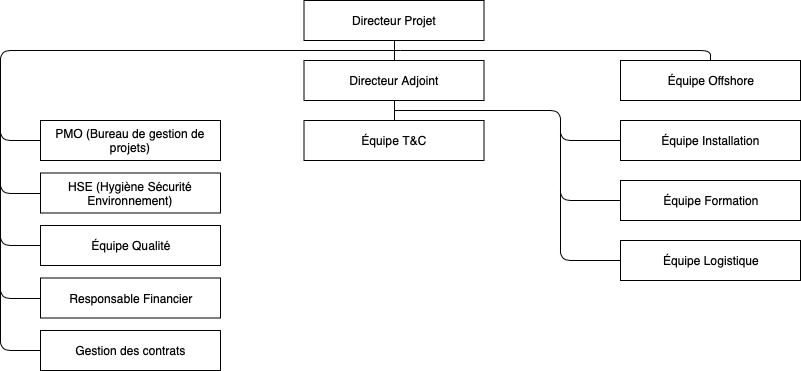
\includegraphics[height=8cm]{ressources/images/figures/OBS1.png}
\end{center}

En ce qui concerne l'équipe \gls{TC} sa fonction principale est de tester et de mettre en service les systèmes et équipements \gls{CCS}.
Son organisation compte environ une trentaine de personnes.
employés est la suivante :

\begin{center}
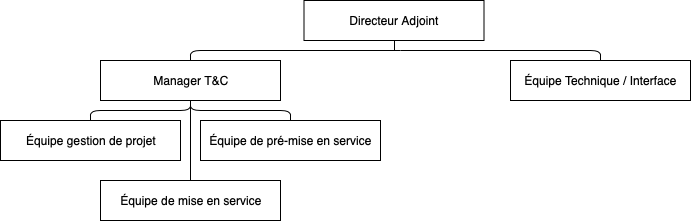
\includegraphics[height=5cm]{ressources/images/figures/OBS2.png}
\end{center}

QDVC est le client direct de Thales mais agit aussi en tant qu'autorité de contrôle durant les différentes phases du projet, en suivant un cycle en V (cf. Annexe I). Concentrons nous ici sur la phase de test : chaque test nécessite le témoignage et l'approbation de QDVC et de ICE, l'entité de contrôle indépendante.
Dans le but de pouvoir mettre en application ce système d'approbation, le client a fait le choix d'une base de donnée permettant l'édition dynamique (et donc la signature) de rapports de test au format pdf : \gls{SnagR}.
Afin d'assurer la communication et le contrôle des documents du référentiel projet, une base de donnée commune est utilisée : \gls{Mezzoteam} mais Thales utilise aussi en parallèle une  base de donnée indépendante du client : \gls{e-TOL}.

Les méthodes utilisée sont les méthodes de gestion de projet dites "classiques", par exemple on peut noter l'utilisation de Primavera, un outil permettant de générer un planning de type Gantt et proposant des outils d'estimation des coûts.
De manière générale, de nombreux outils sont utilisés sur ce projet :
\begin{itemize}
\item \textbf{\gls{Git} :} Outil de gestion des versions et configurations logicielles.
\item \textbf{Doors :} Logiciel de gestion des exigences.
\item \textbf{Giro :} Logiciel de gestion des risques.
\item \textbf{Jira Ops :} Solution de gestion des incidents techniques.
\item \textbf{Palma :} Logiciel de gestion des configurations. 
\end{itemize}

%PRESENTATION TUTEURS

\chapter{Mission}

\section{Sujet du stage}
%Vous présentez le sujet initial tel qu'il a été validé, ses éventuelles évolutions (et leurs causes). Attention, si votre sujet a fortement évolué, vous devez en référer à votre suiveur (éventuellement il devrait être re-validé).
Le sujet de mon stage était la prise en charge du suivi, de la gestion et de l'optimisation  du \gls{reporting} des différents tests de l'équipe \gls{TC}. 
En effet, chaque rapport de test se décompose en plusieurs étapes de test, qui sont toutes reliées à des exigences du cahier des charges. Pour chaque test, QDVC et ICE déterminent si oui ou non les résultats permettent de considérer le rapport comme accepté. Ainsi chaque rapport constitue une preuve nécessaire à la validation des exigences et sans laquelle le système ne peut être validé. 
Chaque rapport est édité et consigné dans la base de donnée \gls{SnagR}. 
Cependant, cet outil est initialement destiné aux projets de génie civil et à la gestion des problèmes d'installation, c'est pour cela que l'utilisation de cet outil a été réduite à l'édition de rapports de test peu de temps après mon arrivée.
Ainsi la problématique initiale fût : Comment suivre efficacement la production et la validation des rapports ?

%Resituer votre sujet dans les objectifs de l'entreprise.
%Avez-vous repris un travail existant ?
%Aviez-vous un cahier des charges précis ou bien avez-vous contribué à son élaboration ?

\section{Planning}
%Vous pouvez présenter le planning initial et le planning réel avec les dates importantes.
En terme de délais, il m'a fallu incorporer les différentes solutions que j'ai mises au point au fur et à mesure du projet, tout en proposition une version finale environ un mois avant la fin de mon stage afin de pouvoir suffisamment l'éprouver.
%Quelles ont été les étapes importantes ? Indiquez celles qui auraient été les plus difficiles, les plus intéressantes, etc.
Le but à court terme était de mettre en place un processus efficace de traitement des rapports et de leurs données puis de l'intégrer au fonctionnement global du projet.
Dans un second temps, le but à long terme était d'automatiser une partie de ce processus, notamment l'extraction et le traitement des données des rapports. 
Enfin, au cours du dernier mois, il m'a fallut former mon remplaçant tant au fonctionnement du \gls{reporting} qu'à l'utilisation des différents outils que j'ai créé.
Chacune de ces trois grandes étapes comporte son lot de difficultés :
\begin{itemize}
\item \textbf{L'initialisation du processus :} L'ampleur du projet constitue une première difficulté. En effet, la tâche qui m'a été confiée demande une bonne connaissance non seulement du fonctionnement interne du projet mais aussi de l'état actuel de son avancement.
\item \textbf{Son automatisation :} La base de donnée avec laquelle je travaillais n'avait pas été documenté, ainsi l'extraction de données s'est avérée complexe.
\item \textbf{Sa transmission :} Former quelqu'un tout en continuant à travailler a constitué un réel défis pour quelqu'un sans expérience professionnelle. 
\end{itemize}
\section{Contributions}
%Quel était l'état du projet à votre arrivée ? et à la fin ?
À mon arrivée, l'installation était arrivée à un stade suffisamment avancé pour permettre de débuter les phases de test (et cela depuis quelques mois).
Ainsi la production des rapports était tout juste amorcée.
C'est pour cela que le projet de mon stage a commencé au moment où on me l'a confié.
À la fin de mon stage, la phase de test était avancée à plus de 50\% et le processus de production et des suivi des rapports de test était en place et fonctionnel.
%Avez-vous travaillé seul ou avec d'autres ? Quelles ont été vos contributions exactes ?
Mes managers m'ont transmis la documentation nécessaire à l'initialisation, de mon projet puis m'ont guidé au cours du stage afin de me permette d'y apporter des améliorations et de nouvelles fonctionnalités. 
Chaque semaine je me devais d'envoyer un rapport sur l'avancement du \gls{reporting} à différents manager Thalès ainsi qu'au client (QDVC).
Ces rapports avaient pour fonction l'aide à la décision et comportaient de nombreux indicateurs d'avancement (\gls{KPI} : Key Progress Indicator).
Je travaillais conjointement avec :
\begin{itemize}
\item Le service de gestion des documents afin de gérer l'indexation des rapports ainsi que leur mise en ligne sur \gls{Mezzoteam} et \gls{e-TOL}.
\item Le service informatique de QDVC afin de proposer des amélioration de la base de données SnagR mais aussi pour leur faire remonter les différentes erreurs de l'interface web.
\item L'équipe \gls{RAMS}  (en français : Fiabilité Maintenabilité Disponibilité et Sécurité), chargée de la sureté de fonctionnement, afin d'effectuer le suivi de la production des documents permettant de prouver la conformité du système en terme de sécurité.
\item L'équipe d'ingénieurs Système, qui est responsable du design, avec qui j'ai étudié différentes exigences.
\item L'équipe d'ingénieurs \gls{TC} afin d'identifier les différents facteurs bloquants ralentissant la production des rapports.
\end{itemize}

%Avez-vous réalisé une étude, une maquette, une preuve de concept, un produit ou une application complète ? Que reste-t-il à faire pour rendre utilisable votre travail ?

En parallèle de ces différentes activités, il m'a fallut automatiser l'extraction des données des rapports. Pour cela j'ai développé un script permettant de se connecter au site \gls{SnagR}, d'en extraire différents lots de données et de les exporter dans différents fichiers Excel. Il m'a fallut aussi ajouter à cette application une fonctionnalité de sauvegarde complète de rapports, en cas de problème avec les serveurs SnagR, serveurs auquel Thalès n'avait pas accès physiquement. 
Ce script est exécutable à travers l'invite de commande, et comme nous le verrons plus tard j'ai formé la personne me remplaçant à son utilisation mais j'ai aussi préparé une documentations. Ainsi, à mon départ, mon remplaçant utilisait déjà les résultats de mon travail.

\section{Technologies}
%Quels sont les outils, environnements ou logiciels que vous avez utilisés ?
Durant mon stage, j'ai donc utilisé : 
\begin{itemize}
\item \textbf{Pour le développement :}
\begin{itemize}
\item \textit{Comme langage de programmation :} Python 2.7 puis Python 3.7.
\item \textit{Comme environnement de développement :} PyCharm, \gls{IDE} de la suite IntelliJ, développé par JetBrains.
\end{itemize}
\item \textbf{Pour la bureautique :} La suite Microsoft Office, plus particulièrement Excel, pour la communication et l'échange d'informations internes au projet, et TexMaker, un éditeur de documents \gls{LaTeX}, pour la rédaction de ce rapport.
\item \textbf{Pour la gestion de mes tâches :} Trello, une solution en ligne de gestion de projet s'inscrivant dans le cadre des \gls{methodesagiles}.
\item \textbf{Pour la gestion des différentes versions du script :} La technologie \gls{Git}, en utilisant l'hébergeur GitHub.
\end{itemize}

%Quelles sont les méthodes utilisées dans votre équipe ? (eg. méthode agile...)
Au sein de l'équipe \gls{TC}, les \gls{methodesagiles} ont été utilisées notamment par le biais d'outils comme \gls{SnagR} ou Jira Ops. En effet, \gls{SnagR} permet aussi de répertorier les problèmes ou points bloquants que les différentes équipes du projet rencontrent. 

\gls{SnagR} est la solution choisie par le Consortium, mais pour son fonctionnement interne, Thales a choisit d'utiliser Jira Ops , qui permet à l'équipe inshore de faire remonter les différents problèmes rencontrés à l'équipe offshore, sous forme de \gls{PCR}.

Parmis ces trois outils que sont SnagR, Jira Ops et Trello \footnote{Jira Ops et Trello sont d'ailleurs édités par la même entreprise : Atlassian} SnagR et Trello intègrent les \gls{methodesagiles}, et plus particulièrement la méthode \textit{KanBan}.

\textbf{La méthode Kanban,} est une méthode de gestion de projet où chaque tâche est placée sur une carte et chaque carte doit être placée dans un tableau. Chaque carte peut être assignée à un ou plusieurs utilisateurs et on peut lui attribuer une date d'échéance ainsi qu'une ou des étiquettes permettant de catégoriser la tâche associée. L'avancement d'une tache est représenté par le déplacement de la carte à laquelle est est liée d'un tableau à un autre. 
En ce qui concerne mon organisation personnelle avec Trello, j'ai utilisé 5 tableaux. Une carte passe successivement par le tableau "À faire", "En cours" puis "Fait" mais peuvent aussi passer par le tableau intermédiaire "En attente" lorsque l'utilisateur nécessite l'achèvement d'une tache par un autre membre du projet, extérieur à l'équipe. À l'exception des taches portant l'étiquette "Récurrente" (étiquette rouge dans l'exemple ci-dessous) qui une fois achevées, retournent dans le tableau "Récurrente".

Voici ci-dessous, l'interface de Trello.

\begin{center}
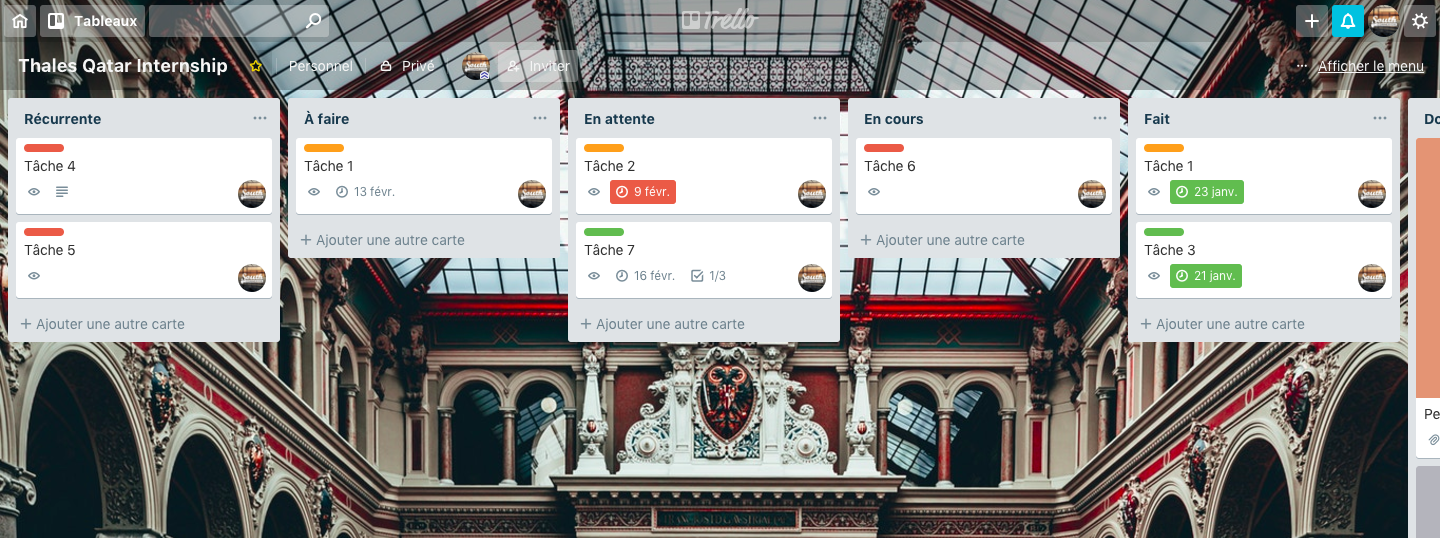
\includegraphics[height=5.5cm]{ressources/images/figures/Trello.png}
\end{center}

\newpage

%Comment les développements ont été vérifiés/testés/validés ?
Concernant le processus que j'ai mis en place, que ce soit pour son initialisation, les différentes modifications apportées à certaines étapes ou l'ajout de certaines étapes, le développement se faisait en 4 étapes :

\begin{itemize}
\item \textit{Formalisation :} Tout d'abord, il fallait analyser le besoin, les ressources dont l'équipe disposait puis chercher une solution optimale et la rendre intelligible afin de pouvoir la communiquer (par le biais d'un diagramme par exemple).
\item \textit{Validation interne :} Ensuite il me fallait exposer ma proposition à mes managers, c'est à dire au directeur adjoint, au manager \gls{TC}, au manager technique et au responsable \gls{RAMS}. Cette étape n'était pas qu'une simple obligation impliquée par le respect de la hiérarchie, elle s'est avérée cruciale par deux aspects majeurs. Tout d'abord, elle permettait de s'assurer de la conformité du processus au regard des besoins de l'équipe. En effet, ces managers possédaient une connaissance poussée des systèmes déployés mais aussi du projet ainsi que du fonctionnement des différentes entités de ce dernier. Ensuite elle était indispensable du point de vue de l'attribution des tâches, afin de ne pas surcharger un employé ou une équipe, ce qui dans un projet de cette envergure, se serait avéré lourd de conséquence. En fonction des remarques et conseils de mes supérieurs, j'effectuais les modifications nécessaires.
\item \textit{Validation externe :} Rendu à ce stade, il fallait ensuite éprouver la solution fasse au client. Non seulement parce qu'il fallait obtenir son accord, mais aussi parce qu'il serait lui aussi concerné par les conséquences de cette décision, étant donné que QDVC et ICE possédaient leurs propres équipes intégrées au processus de \gls{TC}. J'exposerai plus loin les difficultés rencontrées à cette étape.
\item \textit{Application du processus aux équipes \gls{TC} :} Enfin, après avoir obtenu les deux validations nécessaires, il fallait ensuite mettre en place le processus, propager les nouvelles pratiques aux membre des différentes équipes \gls{TC} puis dans un second temps, il me fallait faire remonter aux managers les premiers résultats impliqués par ce changement (nous verrons plus loin les méthodes utilisées).
\end{itemize}

En ce qui concerne l'outil d'automatisation de l'extraction des données que j'ai développé, le processus était identique à l'exception de la validation externe, puisque cette solution était à usage purement interne.
%Quelles sont les technologies utilisées pour le projet ? Il ne s'agit pas de faire de longs développements ici mais de présenter une synthèse.

\section{Prise de recul}
%Quel a été l'intérêt de votre travail pour l'entreprise ? Que va devenir votre contribution ? Présenter les perspectives.

%Quelles sont les améliorations à envisager ? Quelle est la maintenance à prévoir sur cette réalisation ou cette application ?

%Selon les cas, présentez vos réflexions sur l'impact de votre travail sur les utilisateurs, les nouveaux usages, le respect de la vie privée ou de l'environnement...
\chapter{Réalisations}
%Si besoin, vous pourriez structurer le reste du rapport en plusieurs parties et non une seule. La ou les parties devraient elles-mêmes êtres structurées en plusieurs sous-sections au sein d'une même partie. Dans tous les cas, la logique du plan doit apparaître clairement.

%Travaillez les liaisons pour aboutir à une lecture fluide. Voici un exemple (un peu exagéré) : "Après avoir inventorié les technologies disponibles dans la section précédente, cette section est consacrée aux expérimentations que nous avons menées avec chacune d'elles. Ce travail nous permettra de sélectionner les technologies retenues, présentées dans la section suivante."

%Présentez votre réflexion et vos choix, qui devraient être justifiés. Examinez rapidement les autres alternatives.

%Sélectionnez les détails pertinents et laissez les autres en annexe. Allez du général au particulier. Evitez de présenter un catalogue des fonctions développées.

\section{Un stage portée à la fois sur la technique}

\subsection{L'initialisation du processus}

DB, Access, powerbi ou excel ?
=> Limitations dues au caractère sensible des données, process beaucoup trop long

\subsection{Son automatisation}
Pandas

\subsection{Sa transmission}
Multi thread ou multi process ?
=> 

Python 3 ou le choix de la pérénité
=> 2to3

\section{Sur la gestion de projet}

\subsection{Les interactions avec les différentes instances Thales}

\subsection{Celles avec le client}
\chapter*{Conclusion}

\addcontentsline{toc}{chapter}{Conclusion}

%En général, on commence par présenter un résumé du rapport puis les perspectives et éventuellement les travaux restant à mener.
%Vous pouvez ensuite exposer les points positifs et négatifs de votre stage.
%Enfin, vous pouvez re-situer votre stage dans votre parcours de formation et dans votre projet professionnel. Vos objectifs ont-ils évolué ? Par exemple, en quoi ce stage confirme (ou infirme) votre choix de filière ?

Ici j'exposerais : 
\begin{itemize}
\item un résumé du rapport
\item une liste de travaux que j'aurai pus réaliser si j'étais resté plus longtemps (par exemple proposer de mettre l'outil en production en local sur le réseau Thales)
\item les aspects positifs (expérience, communication, etc) et ceux négatifs(gestion de mes tâches pas optimales, mauvaise gestion de mon temps ce qui me faisait travailler le week end ou tard le soir) de mon stage. Je vais reprendre ce que tu (Vincent) avais mis dans ma fiche parce que ça résume bien les difficultés que j'ai eu.
\item Expliquer en quoi ce stage s'est inscrit dans mon parcours : réutilisation des notions et pratiques étudiées en cours et projet (base de donnée, optimisation, gestion de projet etc..)
\item En quoi ce stage a fait évoluer mon projet professionnel donc par exemple : il a renforcé ma motivation a travailler dans l'informatique des réseaux, celle de m'expatrier (volonté d'effectuer un VIE), ma motivation à travailler pour Thales.
\end{itemize}

\printglossary[title={Glossaire}]
\printbibliography[title={Bibliographie},heading={bibintoc}]
\pagenumbering{gobble}

\chapter*{Annexes}
\addcontentsline{toc}{chapter}{Annexes}
%Le lecteur n'est pas obligé de les lire pour évaluer votre travail. Il s'agit d'un complément auquel pourrait se reporter le lecteur.
%Par exemple, vous pourriez mettre une copie d'écran, un extrait de code, etc. Gardez à l'esprit que le lecteur devrait comprendre le rapport sans se reporter aux annexes. Si ce n'est pas le cas, alors l'information devrait apparaître dans le corps du rapport et non en annexe.
%Dans tous les cas, les annexes doivent être citées dans le corps du rapport. Par exemple: "(cf. annexe XX)" ou "Pour plus de détails, le lecteur pourra se reporter à l'annexe XX page XX."

\subsection*{Annexe I - Cycle de développement (en V) }

%\begin{center}
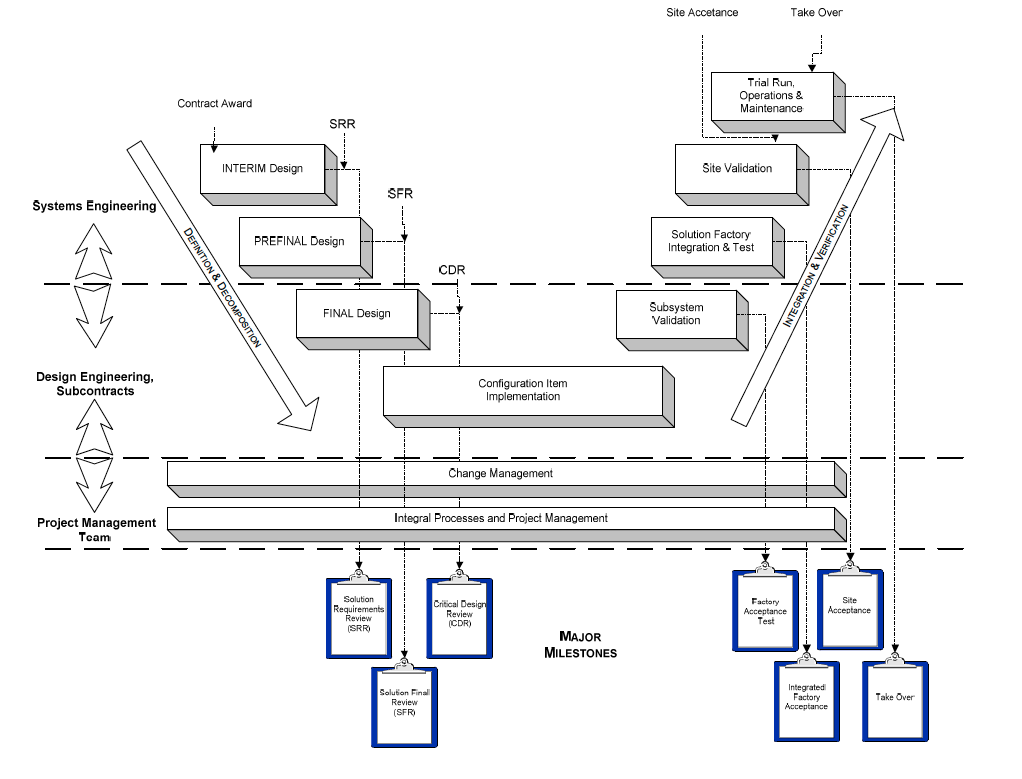
\includegraphics[height=14cm]{ressources/images/annexes/Vcycle.png}
%\end{center}


\end{document}
\grid
